%%%%%%%%%%%%%%%%%%%%%%%%%%%%%%%%%%%%%%%%%
% Short Sectioned Assignment
% LaTeX Template
% Version 1.0 (5/5/12)
%
% This template has been downloaded from:
% http://www.LaTeXTemplates.com
%
% Original author:
% Frits Wenneker (http://www.howtotex.com)
%
% License:
% CC BY-NC-SA 3.0 (http://creativecommons.org/licenses/by-nc-sa/3.0/)
%
%%%%%%%%%%%%%%%%%%%%%%%%%%%%%%%%%%%%%%%%%

%----------------------------------------------------------------------------------------
%	PACKAGES AND OTHER DOCUMENT CONFIGURATIONS
%----------------------------------------------------------------------------------------

\documentclass[paper=a4, fontsize=11pt]{scrartcl} % A4 paper and 11pt font size

\usepackage[T1]{fontenc} % Use 8-bit encoding that has 256 glyphs
\usepackage{setspace}
\doublespacing
\usepackage{palatino}
\usepackage{rotating}
%\usepackage{Georgia} % Use the Adobe Utopia font for the document - comment this line to return to the LaTeX default
\usepackage[english]{babel} % English language/hyphenation
\usepackage{amsmath,amsfonts,amsthm} % Math

\usepackage{lipsum} % Used for inserting dummy 'Lorem ipsum' text into the template

\usepackage{sectsty} % Allows customizing section commands
\allsectionsfont{\centering \normalfont\scshape} % Make all sections centered, the default font and small caps

\usepackage{fancyhdr} % Custom headers and footers
\pagestyle{fancyplain} % Makes all pages in the document conform to the custom headers and footers
\fancyhead{} % No page header - if you want one, create it in the same way as the footers below
\fancyfoot[L]{} % Empty left footer
\fancyfoot[C]{} % Empty center footer
\fancyfoot[R]{\thepage} % Page numbering for right footer
\renewcommand{\headrulewidth}{0pt} % Remove header underlines
\renewcommand{\footrulewidth}{0pt} % Remove footer underlines
\setlength{\headheight}{13.6pt} % Customize the height of the header

\numberwithin{equation}{section} % Number equations within sections (i.e. 1.1, 1.2, 2.1, 2.2 instead of 1, 2, 3, 4)
\numberwithin{figure}{section} % Number figures within sections (i.e. 1.1, 1.2, 2.1, 2.2 instead of 1, 2, 3, 4)
\numberwithin{table}{section} % Number tables within sections (i.e. 1.1, 1.2, 2.1, 2.2 instead of 1, 2, 3, 4)

\setlength\parindent{0pt} % Removes all indentation from paragraphs - comment this line for an assignment with lots of text

%----------------------------------------------------------------------------------------
%	TITLE SECTION
%----------------------------------------------------------------------------------------

\newcommand{\horrule}[1]{\rule{\linewidth}{#1}} % Create horizontal rule command with 1 argument of height

\title{
\normalfont \normalsize
\textsc{University of Windsor, Department of civil and environmental engineering} \\ [25pt] % Your university, school and/or department name(s)
\horrule{0.5pt} \\[0.4cm] % Thin top horizontal rule
\huge Spring Calculation \\ % The assignment title
\horrule{2pt} \\[0.5cm] % Thick bottom horizontal rule
}

\author{Ran Wang} % Your name

\date{\normalsize\today} % Today's date or a custom date

\begin{document}

\maketitle % Print the title

%----------------------------------------------------------------------------------------
%	Question 1
%----------------------------------------------------------------------------------------

\section{Analytical Model}

In-plane and out-of-plane are two vibration forms commonly observed
on-site for the cable-stayed bridges. This project aims to find a
relationship between the stiffness the spring of the supporting system
with the natural frequency of the cables. To have a better understand
of the underlying mechanism of the instability, a
two-degree-of-freedom model will be developed. However, one should
keep in mind that the dynamic response of the system also affected by
how many degrees of freedom. This project is just a basic calculation
to determine the stiffness of springs.

First, the in-plane motion can be model as a rigid bar of total mass (m)
sitting on two springs with stiffness (k) shown in the Figure 1. Damping
effects and pretension of the cable are ignored. This rigid bar is
constrained such that only the vertically movement is allowed. In
other word, no vibrations will occur in the out-of-plane. This is a
typical two degrees-of-freedom system.

\begin{figure}
  \centering
  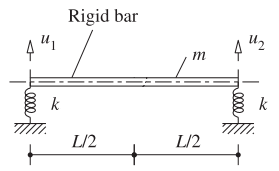
\includegraphics[width=0.4\linewidth]{fig/ana-mode.png}
\end{figure}

The system is a localized stiffness with distributed mass system.
Since the springs are defined at the degree-of-freedom, so the
stiffness matrix of the system can be written as:

\begin{align}
  k=\ \left[\begin{matrix}k&0\\0&k\\\end{matrix}\right].
\end{align}

To obtain the mass matrix, one should impart a unit acceleration at
degree of freedom 1 with zero acceleration at degree-of-freedom 2. By
considering the inertia force, one can calculate $m_{11}$ and $m_{21}$
equal to $\frac{m}{3}$ and $\frac{m}{6}$ , respectively. Similarly, by
applying a unit acceleration at degree-of-freedom 1, $m_{12}$ and $m_{22}$
can be calculated as $\frac{m}{6}$ and $\frac{m}{3}$ , respectively. Thus,
the mass matrix can be set up as:

\begin{align}
  m=\frac{m}{6}\ \left[\begin{matrix}2&1\\1&2\\\end{matrix}\right].
\end{align}

Once the stiffness matrix and mass matrix are determined, the equation
of motion can be written as:

\begin{align}
\frac{m}{6}\
  \left[\begin{matrix}2&1\\1&2\\\end{matrix}\right]\left[\begin{matrix}{\ddot{u}}_1\\{\ddot{u}}_2\\\end{matrix}\right]+\
  \left[\begin{matrix}k&0\\0&k\\\end{matrix}\right]\left[\begin{matrix}u_1\\u_2\\\end{matrix}\right]=\left[\begin{matrix}0\\0\\\end{matrix}\right].\
\end{align}

The motion of the sytem for single degree-of-freedom is known as
simple harmonic motion. By solving the above linear sytem, one can
determine the circular frequencies of the system:

\begin{align}
  \begin{bmatrix}\omega_1\\\omega_2\\\end{bmatrix} =
  \begin{bmatrix} \sqrt{\frac{2k}{m}} \\ \sqrt{\frac{6k}{m}} \\ \end{bmatrix}.
\end{align}

Model parameters can be found in Table 1.1.

\begin{table}
  \centering
  \begin{tabular}{ll}
    \hline    
    Length	&   1.4 $m$ \\
    Out diameter of the cable &	0.0889 $m$ \\
    Inner diameter of the cable &	0.0762 $m$ \\
    Young's Modulus	& 3.2E9 $Pa$\\
    Density of the cable & 	 1163 $Kg/m^{3}$\\
    Stiffness of the spring	 &  3 $N/m$ \\
    \hline
  \end{tabular}
  \caption{Parameters of the cable model.}
  \label{tab:cable-parameter}
\end{table}

Finally, the natral frequencies of the system are determined:

\begin{align}
\left[\begin{matrix}f_1\\f_2\\\end{matrix}\right]=\left[\begin{matrix}0.2381\\0.4125\\\end{matrix}\right]
  Hz.\\
\end{align}

%% raw calculation
% outer pi (D/2)^2 = 3.14 * (0.0889/2)^2 = 6.20401985e-3
% inner pi (D/2)^2 = 3.14 * (0.0762/2)^2 = 4.5580554e-3

% 2D Area = 6.20401985e-3 - 4.5580554e-3 = 1.64596445e-3

% Volume  = 1.64596445e-3 * 1.4 = 2.30435023e-3 m^3

% Mass    = 2.30435023e-3 * 1163 = 2.67995931749 kg

% sqrt(2*3 / 2.68) = 1.49626400416

% f = 1.49626400416 / (2 pi) =  1.49626400416 / (2*3.14) =
% 0.238258599389 Hz

It should be noted that modal shape corresponding to the fundamental
frequency is that two ends of the cable segments moving
simultaneously, whereas the second modal shape represents that two
ends of the cable moving out-of-phase.

\section{Finite Element Model}
\label{sec:finite-element-model}

\subsection{Modal Analysis}
\label{sec:modal-analysis}

Modal analysis is the process of determining the inherent dynamic
characteristics of a system in forms of natural frequencies, damping
factors and mode shapes, and using them to formulate a mathematical
model for its dynamic behavior(He, Fu, and Fu 2001).

The dynamics responses of the system are decomposed by frequency and
corresponding position. This kind of analysis can be verified from
analytical solutions of partial differtial equation for some simple
geometries. The mathematic fundation of this theory is based on that
the response of of a linear system can be written as a series of
harmonic movments. Mathematically speaking, any complicated function
can be expressed in sets of sine or consine functions using Fourier
transform. The concept of modal analysis is similar with that
mathematic concept. The natural modes of a given system are determined
once its physical properties such as mass, stiffness and damping and
spatial distribution. The parameters such as natural frequency and
moda shape are used to describe the system movment.

Modal analysis includes both theoretical and experimental approaches.
Besides the theoretical manipulations of equations, with the rapid
progress of data acquisition technolgies, the modal testing is becoming
more and more popular to determine the natural frequency of a system.

In this project, a commerical software Abaqus 6.14 is utilized to
analyse modal response of the cable. The purpose of the simulation is
to compare hand calculations with numerical simulations. Once the
validation is done, one can further investigate problems that are hard
to calculate using analytical solution.

Wilkinson and Wilkinson (1965) detailed the problems in his book. The
reason why eigenvale problem is popular with finite element analysis
is that these problems involve large but narrowly banded matrices. The
matrices of majority problems are symmetry. A typtical mathematical
description of the problem is:

\begin{align}
\left(\mu^2\left[M\right]+\mu\left[C\right]+\left[K\right]\right)\left\{\psi\right\}=0,
\end{align}

where $[M]$ is the mass matrix, which is symmetry and postive define;
$[C]$ is the damping matrix; $[K]$ is the stiffness matrix, which may
include large-displacment effects, and, therefore, may not always be
positive definite or sysmmetry; $\mu$ is the eigenvalue;
$\left\{\psi\right\}$ is the eigenvetor-the mode shape of motion;

The eigensystem have complex eigenvalues and eigenvectors in general.
The system can be symmetrized by assuming $[K]$ is symmetry and neglect
damping matrix during analysis. For a symmetic eigenproblem, assuming
$[K]$ is also positive semidefinite. In this case $\mu$ becomes an
imaginery eigenvalue, $\mu=i\omega$, where $\omega$ is the circular
frequey of the system, so the system can be rewriten as:

\begin{align}
\left(-\omega^2\left[M\right]+\left[k\right]\right)\left\{\psi\right\}=0.
\end{align}

Abaqus provides eignevalue extration procedures for above system. For
symmetrized eigenvalue problems Abaqus offers two methods: Lanczos and
subspace iteration methods.The solver using in this project is called
Lanczos eigensolver. This kind of algorithem is powerful in extration
of the extreme eigenvalues and the corresponding eigenvectors.

\subsection{FEM Modeling}
\label{sec:fem-modeling}

In the part, materials and sections models, the geometry and physical
properties are defined. In the step setting, non-linear effect is
ignored; Lanczos eigensolver is choosen. C3D8R element is used to
discretize the whole system. Since the analytical solution is provided
in the previous discussion, there is no need to do mesh independent
study. Boundary condtions are defined in such a way that it is very
simlary to hand calculation. The cable is connected with two springs.
The cable is simulated as a rigid bar. The only difference is that the
cable is allowed to have axial displacement, in order to obtain the
second modal shape from hand calculations.

Boundary condtions are defined in such a way that it is very simlary
to hand calculation. The cable is connected with two springs. The
cable is simulated as a rigid bar. The only difference is that the
cable is allowed to have axial displacement, in order to obtain the
second modal shape from hand calculations.

\subsection{FEA Results}
\label{sec:fea-results}

The simulaiton result is present in the Table 2.1 It shows that the two
calculations agree with each other very well, thus the calculation of
the natural frequency of the cable is reasonable using the simplified
assumptions.

\begin{table}
  \centering
  \begin{tabular}{lll}
    \hline    
   & Hand Calculation &FEA \\
   f1&	0.2381&	0.2375 \\
    f2&	0.4125&	0.4102 \\
    \hline
  \end{tabular}
  \caption{Comparison of hand calculation and FEA result.}
\end{table}

\newpage
\begin{sidewaysfigure}
\begin{verbatim}
                              E I G E N V A L U E    O U T P U T     

 MODE NO      EIGENVALUE              FREQUENCY         GENERALIZED MASS   COMPOSITE MODAL DAMPING            
                             (RAD/TIME)   (CYCLES/TIME)


       1*    -9.45461E-07     0.0000         0.0000         2.3422         0.0000    
       2*    -7.89616E-08     0.0000         0.0000         2.6946         0.0000    
       3       2.2268         1.4922        0.23750         2.6943         0.0000    
       4       6.6446         2.5777        0.41025        0.90300         0.0000    
       5       56216.         237.10         37.735         1.3560         0.0000    
       6      2.86499E+05     535.26         85.189        0.69476         0.0000    
       7      8.14360E+05     902.42         143.62         1.3805         0.0000    
       8      2.00447E+06     1415.8         225.33        0.73256         0.0000    
       9      2.41443E+06     1553.8         247.30        0.85643         0.0000    
      10      2.60206E+06     1613.1         256.73        0.85578         0.0000    

 ***NOTE: EIGENVALUES MARKED WITH A * APPEAR TO BE RIGID BODY MODES
\end{verbatim}
\end{sidewaysfigure}

\section{Design VIV spring}
\label{sec:design-viv-spring}

The natural frequency is calculated as:

\begin{align}
f = \sqrt{\frac{2k}{m}} / 2 \pi.
\end{align}

Therefore, stiffness is a function of natural frequency:
\begin{align}
  k &= 2 \pi^2 m f^2, or \\
    &=  2 * 3.1416 * 3.1416 * 2.67 f^2 \\
    &=  52.7 f^2
\end{align}

Given the Strouhal number $(St = f D/U)$ as a constant number 0.21 and
wind speed $(10 m/s)$ in the wind tunnel, the VIV frequency is
calculated as:
\begin{align}
  f &= 0.21 U /D \\
    &= 0.21 * 10 / 0.0889 \\
    &= 23.622 (Hz).
\end{align}

Based on these assumptions, we can calculate the stiffness of the
spring:
\begin{align}
  k    &=  52.7 f^2 \\
       &=  52.7 * 23.622^2 \\
       &=  29406 N/m
\end{align}

  % Free-stream fluid velocity:	   10 m/s
   
  % Characteristic distanceD:	   0.0889 m
   
  % Fluid density,	   1.25 kg/m3
   
  % Fluid viscosity (dynamic):	   1.8E-005 Pa-s
   
\end{document}

%%% Local Variables:
%%% mode: latex
%%% TeX-master: t
%%% End:
